\documentclass{article}
\usepackage[utf8]{inputenc}
\usepackage[includeheadfoot, margin=1em,headheight=2em]{geometry}
\usepackage{titling}
\geometry{a4paper, left=2cm, right=2cm, top=2cm, bottom=2cm}
\usepackage{graphicx}
\usepackage{hyperref}
\usepackage{url}
\usepackage{enumitem}
\providecommand{\versionnumber}{1.3.0}
\usepackage{array}
\usepackage[italian]{babel}
\newcolumntype{P}[1]{>{\centering\arraybackslash}p{#1}}
\renewcommand{\arraystretch}{1.5} % Default value: 1
\setlength{\droptitle}{-6em}
\usepackage{capt-of}
\usepackage{float}


%font
\usepackage[defaultfam,tabular,lining]{montserrat}
\usepackage[T1]{fontenc}
\renewcommand*\oldstylenums[1]{{\fontfamily{Montserrat-TOsF}\selectfont #1}}

%custom bold 
\usepackage[outline]{contour}
\usepackage{xcolor}
\newcommand{\custombold}{\contour{black}}

%table colors
\usepackage{color, colortbl}
\definecolor{Blue}{rgb}{0.51,0.68,0.79}
\definecolor{LightBlue}{rgb}{0.82,0.87,0.90}
\definecolor{LighterBlue}{rgb}{0.93,0.95,0.96}

%Header
\usepackage{fancyhdr, xcolor}
\pagestyle{fancy}
\let\oldheadrule\headrule% Copy \headrule into \oldheadrule
\renewcommand{\headrule}{\color{Blue}\oldheadrule}% Add colour to \headrule
\renewcommand{\headrulewidth}{0.2em}
\fancyhead[L]{Analisi dei requisiti}
\fancyhead[C]{Cybersorceres}
\fancyhead[R]{versione \versionnumber}


\title{\Huge{\textbf{Analisi dei requisiti}}\vspace{-1em}}

\author{CyberSorcerers Team}
\date{}

 % Imposta labelformat=empty per nascondere il prefisso "Figura X:"
 \usepackage{caption}
\captionsetup[figure]{labelformat=empty}

\begin{document}
\maketitle

\vspace{-3em}
\begin{figure}[h]
  \centering
  
\includegraphics[width=6cm, height=6cm]{documenti/logo rotondo.png}
  \label{fig:immagine}
\end{figure}

\vspace{6em}
\large{

\begin{center}
    \begin{tabular}{l c c}
        \rowcolor{Blue} 
        \textbf{Informazioni sul documento} & &\\ [1 ex]
        \rowcolor{LighterBlue}
        Destinatari: & Prf. Tullio Vardanega & Prf. Riccardo Cardin\\ [1 ex]
        \rowcolor{LightBlue}
        G al pedice: & Consultare il Glossario & \\ [1 ex]
    \end{tabular}
\end{center}}

\begin{table}[h]
\centering
\begin{tabular}{c}
\rowcolor{Blue}
\textbf{Membri del team} \\
\rowcolor{LighterBlue}
Samuele Vignotto \\
\rowcolor{LightBlue}
Giulia Dentone \\
\rowcolor{LighterBlue}
Andrea Rezzi \\
\rowcolor{LightBlue}
Giovanni Moretti \\
\rowcolor{LighterBlue}
Sabrina Caniato \\
\rowcolor{LightBlue}
Nicola Lazzarin \\
\end{tabular}
\end{table}

\newpage
\custombold{Registro dei Cambiamenti - Changelog\textsubscript{G}}

\begin{center}
\begin{tabular}{P{4em} P{6em} P{7em} P{7em} P{11em}} 
  \rowcolor{Blue}
    \custombold{Versione} & \custombold{Data} & \custombold{Autore} &
    \custombold{ Verificatore} & \custombold{Dettaglio}\\
    \rowcolor{LighterBlue}
    1.3.0 & 25/04/2024 & Samuele Vignotto & Giulia Dentone & Correzione UC fino a UC21.\\
    \rowcolor{LightBlue}
    1.2.0 & 23/04/2024 & Giulia Dentone & Samuele Vignotto & Aggiunta UC1 e correzione fino a UC7.\\
    \rowcolor{LighterBlue}
    1.1.0 & 17/04/2024 & Samuele Vignotto & Giulia Dentone & Correzione scenari principali e inizio correzioni esito RTB.\\
    \rowcolor{LightBlue}
    1.0.0 & 05/04/2024 & Giulia Dentone & Samuele Vignotto & Revisione finale del documento.\\
    \rowcolor{LighterBlue}
    0.9.2 & 07/03/2024 & Samuele Vignotto & Sabrina Caniato & Aggiunta ultimi requisiti individuati durante ultima riunione esterna e verifica.\\
    \rowcolor{LightBlue}
    0.9.1 & 06/03/2024 & Samuele Vignotto & Giulia Dentone & Aggiunta di requisiti da Capitolato.\\
    \rowcolor{LighterBlue}
    0.9.0 & 09/12/2023 & Nicola Lazzarin & Sabrina Caniato & Inserimento dei requisiti prestazionali.\\
    \rowcolor{LightBlue}
    0.8.2 & 09/12/2023 & Nicola Lazzarin & Sabrina Caniato & Update dei requisiti di vincolo.\\
    \rowcolor{LighterBlue}
    0.8.1 & 06/12/2023 & Samuele Vignotto & Giulia Dentone & Update dei requisiti di vincolo.\\
    \rowcolor{LightBlue}
    0.8.0 & 05/12/2023 & Samuele Vignotto & Nicola Lazzarin & Aggiunta dei requisiti di vincolo.\\
    \rowcolor{LighterBlue}
    0.7.0 & 04/12/2023 & Giulia Dentone & Nicola Lazzarin & Aggiunta dei requisiti di qualità.\\
    \rowcolor{LightBlue}
    0.6.0 & 03/12/2023 & Samuele Vignotto & Sabrina Caniato & Aggiunta dei requisiti funzionali.\\
    \rowcolor{LighterBlue}
    0.5.2 & 03/12/2023 & Samuele Vignotto & Sabrina Caniato & Aggiunta fonti requisiti.\\
    \rowcolor{LightBlue}
    0.5.1 & 02/12/2023 & Nicola Lazzarin & Giulia Dentone & Aggiunta caption alle immagini.\\ 
    
    \end{tabular}


\begin{tabular}{P{4em} P{6em} P{7em} P{7em} P{11em}} 
    \rowcolor{LighterBlue}
    0.5.0 & 01/12/2023 & Caniato Sabrina & Vignotto Samuele & Sistemato l'analisi dei casi d'uso\textsubscript{G} dopo il colloquio col Prof. R. Cardin. Aggiunta delle specifiche dei sottocasi d'uso.\\
    \rowcolor{LightBlue}
    0.4.3 & 30/11/2023 & Sabrina Caniato & Samuele Vignotto & Inserimento delle immagini relative dall'UC14 all'UC18.\\
    \rowcolor{LighterBlue}
    0.4.2 & 28/11/2023 & Giulia Dentone & Nicola Lazzarin & Inserimento delle immagini relative dall'UC7 all'UC14.\\
    \rowcolor{LightBlue}
    0.4.1 & 27/11/2023 & Sabrina Caniato & Nicola Lazzarin & Inserimento delle immagini relative dall'UC1 all'UC6.\\
    \rowcolor{LighterBlue}
    0.4.0 & 27/11/2023 & Nicola Lazzarin & Samuele Vignotto & Descrizione tesuale dall'UC16 all'UC18. \\
    \rowcolor{LightBlue}
    0.3.0 & 25/11/2023 & Sabrina Caniato & Samuele Vignotto & Descrizione tesuale dall'UC11 all'UC15. \\
   \rowcolor{LightBlue}
    0.2.0 & 24/11/2023 & Giulia Dentone & Samuele Vignotto & Descrizione testuale dall'UC6 all'UC10.\\ 
    \rowcolor{LighterBlue}
    0.1.0 & 23/11/2023 & Giulia Dentone & Sabrina Caniato & Descrizione testuale dall'UC1 all'UC5.\\
    \rowcolor{LightBlue}
    0.0.1 & 23/11/2023 & Caniato Sabrina  & Samuele Vignotto & Definizione struttura del documento e scheletro delle sezioni. Scrittura introduzione ed obiettivi delle diverse sezioni.\\ 
\end{tabular}
\end{center}
\newpage
\tableofcontents
\listoffigures
\listoftables
\newpage
\section*{Introduzione}

\subsection*{Scopo del documento}

Questo documento ha lo scopo di fornire una descrizione approfondita del prodotto, analizzando nel dettaglio i requisiti, ottenuti tramite incontri con l'azienda e analisi del capitolato. Quest'analisi si concretizza con l'individuazione di casi d'uso\textsubscript{G}, punto centrale di questo documento.


\subsection*{Scopo del prodotto}
L'azienda proponente ha richiesto la creazione di una web app\textsubscript{G} che, tramite l'uso di IA\textsubscript{G} (in questo caso ChatGPT4 e Bedrock) è in grado di creare epic user stories\textsubscript{G} a partire dalle richieste del cliente e confrontarle con il codice sviluppato in modo da informare il cliente dello stato di avanzamento dello sviluppo del prodotto. Inoltre deve essere possibile, sia per il Project Manager\textsubscript{G}, sia per il cliente rilasciare dei feedback (nel primo caso riguardanti l'adeguatezza delle stories, nel secondo caso riguardanti il prodotto finale) al fine di migliorare l'IA\textsubscript{G}. È inoltre richiesta un' analisi comparativa tra le due IA\textsubscript{G} utilizzate e lo sviluppo di un plug-in\textsubscript{G} utile agli sviluppatori e al Project Manager\textsubscript{G}.

\subsection*{Glossario}
Alcuni termini presenti nel documento potrebbero essere ambigui, pertanto verranno inseriti nel Glossario v.1.0.0. La loro presenza all'interno di esso sarà indicata tramite una G maiuscola a pedice.

\subsection*{Riferimenti}
\subsubsection{Riferimenti normativi}
\begin{itemize}
    \item Capitolato \textbf{C7 - ChatGPT vs BedRock developer Analysis}
    \\ \\
       \href{https://github.com/CyberSorceres/CyberSorceresRepository}{https://github.com/CyberSorceres/CyberSorceresRepository} 
    \item Norme del way of working v 1.0.0
    \item Regolamento del progetto didattico \\ \\ \href{https://www.math.unipd.it/~tullio/IS-1/2023/Dispense/PD2.pdf} 
    {https://www.math.unipd.it/~tullio/IS-1/2023/Dispense/PD2.pdf}
\end{itemize}

\subsubsection{Riferimenti informativi}
\begin{itemize}
    \item Lezione del corso di Ingegneria del software "Analisi e descrizione delle funzionalità: Use Case e relativi diagrammi (UML)" \url{https://www.math.unipd.it/~rcardin/swea/2022/Diagrammi%20Use%20Case.pdf}
    \item Lezione del corso di Ingegneria del software "Analisi dei requisiti (T5)" \\ \\
    \url{https://www.math.unipd.it/~tullio/IS-1/2023/Dispense/T5.pdf}
    
    

\end{itemize}


\section*{Casi d'uso}
\subsection*{Scopo}
Lo scopo di questa sezione è raccogliere tutti i casi d'uso\textsubscript{G} individuati, facendo riferimento alle funzionalità individuate durante la sessione di design thinking\textsubscript{G} fatta in collaborazione con l'azienda.

\subsection*{Attori}
Come si è evidenziato durante la sessione di design thinking\textsubscript{G} con i proponenti la web app\textsubscript{G} avrà necessità di tre diverse interfacce per essere usata adeguatamente da tutte le tipologie di attori\textsubscript{G}: clienti, sviluppatori e Project Manager\textsubscript{G}. L'IA\textsubscript{G}  (ChatGPT o Bedrock) viene considerata attore\textsubscript{G} secondario in quanto utilizzeremo un servizio che ci viene offerto. Inoltre è necessario lo sviluppo di un plug-in\textsubscript{G} accessibile solamente a agli sviluppatori e al Project Manager\textsubscript{G}.\\\\

Per facilitare la comprensione del diagramma dei casi d'uso\textsubscript{G}  abbiamo utilizzato due generalizzazioni: Utente e Utente aziendale: 

\begin{figure}[h]
    \centering
    \includegraphics{documenti/imgUML/Attori.png}
    \caption{Generalizzazione degli attori\textsubscript{G} Utente ed Utente Aziendale}
    \label{fig:attori}
\end{figure}

\newpage
\custombold{UML Casi d'uso}
\begin{figure}[h]
    \centering
    \includegraphics[height = 0.70\textheight]{documenti/imgUML/UML.png}
    \caption{UML dei casi d'uso\textsubscript{G}}
    \label{fig:UML}
\end{figure}
\newpage

\section{UC1-Registrazione}
    \begin{figure}[h]
      \centering
      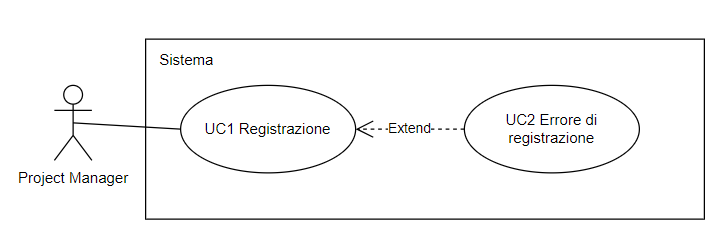
\includegraphics{documenti/imgUML/UC1-REGISTRAZIONE.png}
      \caption{UC1}
      \label{fig:UC1}
    \end{figure}  

         \subsection*{Main actor}
         \begin{itemize}
             \item Project Manager\textsubscript{G}.
         \end{itemize}
     \subsection*{Preconditions} 
        \begin{itemize}
            \item Essere registrati nel sistema come Project Manager\textsubscript{G} con i propri permessi.
        \end{itemize}
            \subsection*{Postconditions}
        \begin{itemize}
            \item Project Manager\textsubscript{G} riconosciuto dal sistema;
            \item Nuovo utente inserito nel sistema.
        \end{itemize}
    \subsection*{Main scenario}
   \begin{figure}[H]
      \centering
      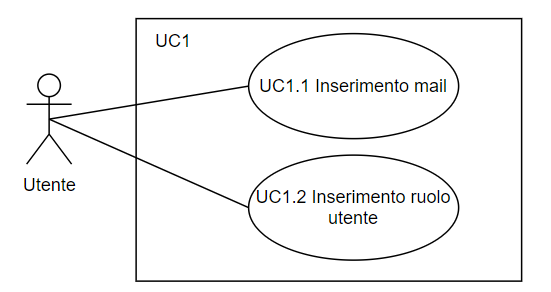
\includegraphics{documenti/imgUML/UC1-SOTTOCASI.png}
      \caption{UC1.1 e UC1.2}
      \label{fig:UC1,1 e UC1.2}
    \end{figure} 
        \begin{itemize}
            \item Inserimento manuale della mail dell'utente;
            \item Inserimento del ruolo dell'utente (Cliente, Sviluppatore, Project Manager\textsubscript{G}).
        \end{itemize}
    \subsection*{Alternative scenario}
        \begin{itemize}
            \item Visualizzazione del messaggio di errore per un utente già inserito nel sistema [UC2].
        \end{itemize}

\subsection{UC1.1-Inserimento Mail}
    
     \subsection*{Main actor}
         \begin{itemize}
             \item Project Manager\textsubscript{G}.
         \end{itemize}
     \subsection*{Preconditions} 
        \begin{itemize}
            \item Essere registrati nel sistema con i propri permessi;
        \end{itemize}
        \subsection*{Postcondition} 
        \begin{itemize}
            \item Email dell'utente inserita.
        \end{itemize}
        \subsection*{Main scenario}
        \begin{itemize}
        \item Compilazione campo mail.
        \end{itemize}

\subsection{UC1.1-Inserimento Ruolo}
    
     \subsection*{Main actor}
         \begin{itemize}
             \item Project Manager\textsubscript{G}.
         \end{itemize}
     \subsection*{Preconditions} 
        \begin{itemize}
            \item Essere registrati nel sistema con i propri permessi;
        \end{itemize}
        \subsection*{Postcondition} 
        \begin{itemize}
            \item Ruolo dell'utente inserito (Cliente, sviluppatore, Project Manager\textsubscript{G}).
        \end{itemize}
        \subsection*{Main scenario}
        \begin{itemize}
        \item Compilazione del campo ruolo.
        \end{itemize}

\section{UC2-Errore di registrazione}
    \subsection*{Main actor}
         \begin{itemize}
             \item Project Manager\textsubscript{G}.
         \end{itemize}
         
     \subsection*{Preconditions} 
        \begin{itemize}
            \item Essere registrati nel sistema con i propri permessi.
        \end{itemize}
        
    \subsection*{Postconditions}
        \begin{itemize}
            \item Utente già presente nel sistema.
        \end{itemize}
        \subsection*{Main scenario}
        \begin{itemize}
        \item Inserimento della mail dell'utente da inserire;
        \item Inserimento del ruolo dell'utente da inserire (Cliente, Sviluppatore, Project Manager).
        \end{itemize}

\section{UC3-Autenticazione}
    \begin{figure}[h]
      \centering
      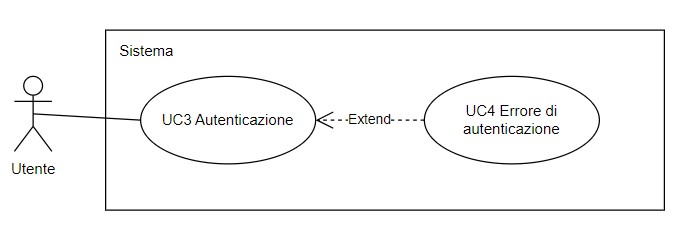
\includegraphics{documenti/imgUML/UC3-AUTENTICAZIONE.png}
      \caption{UC3 e UC4}
      \label{fig:UC3 AUTENTICAZIONE}
    \end{figure} 
    
     \subsection*{Main actor}
         \begin{itemize}
             \item Utente.
         \end{itemize}
     \subsection*{Preconditions} 
        \begin{itemize}
            \item Essere registrati nel sistema con i propri permessi.
        \end{itemize}
               
    \subsection*{Postconditions}
        \begin{itemize}
            \item Utente riconosciuto dal sistema.
        \end{itemize}
    \subsection*{Main scenario}
        \begin{figure}[h]
            \centering
            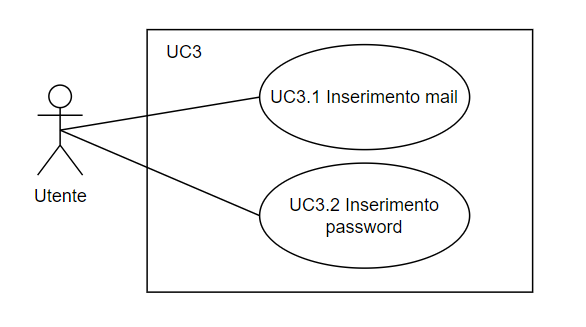
\includegraphics{documenti/imgUML/UC3-SOTTOCASI.png}
            \caption{UC3.1 e UC3.2}
            \label{fig:UC3 SOTTOCASI}
        \end{figure}
        \begin{itemize}
            \item Compilazione campo mail [UC1.1];
            \item Compilazione campo password [UC1.2].
        \end{itemize}
            
        \subsection*{Alternative scenario}
            \begin{itemize}
                \item Visualizzazione errore di autenticazione [UC4].
            \end{itemize}
            
\subsection{UC3.1-Inserimento Mail}
    
     \subsection*{Main actor}
         \begin{itemize}
             \item Utente.
         \end{itemize}
     \subsection*{Preconditions} 
        \begin{itemize}
            \item Essere registrati nel sistema con i propri permessi;
            \item Trovarsi nella pagina di login.
        \end{itemize}
        \subsection*{Postcondition} 
        \begin{itemize}
            \item Email inserita.
        \end{itemize}
        \subsection*{Main scenario}
        \begin{itemize}
        \item Compilazione campo mail.
        \end{itemize}

\subsection{UC3.2-Inserimento Password}
    
     \subsection*{Main actor}
         \begin{itemize}
             \item Utente.
         \end{itemize}
     \subsection*{Preconditions} 
        \begin{itemize}
            \item Essere registrati nel sistema con i propri permessi;
            \item Trovarsi nella pagina di login.
        \end{itemize}
        \subsection*{Postcondition} 
        \begin{itemize}
            \item Password inserita;
            \item Possibilità di effettuare il login.
        \end{itemize}
         \subsection*{Main scenario}
        \begin{itemize}
        \item Compilazione campo password.
        \end{itemize}

\section{UC4-Errore di autenticazione}
    
     \subsection*{Main actor}
         \begin{itemize}
             \item Utente.
         \end{itemize}
     \subsection*{Preconditions} 
        \begin{itemize}
            \item Essere registrati nel sistema con i propri permessi.
        \end{itemize}
               
    \subsection*{Postconditions}
        \begin{itemize}
            \item Utente Non riconosciuto dal sistema.
        \end{itemize}
        \subsection*{Main scenario}
        \begin{itemize}
        \item Inserimento della password;
        \item Inserimento della mail.
        \end{itemize}

    
\section{UC5-Compilazione requisiti di business}
    \begin{figure}[H]
      \centering
      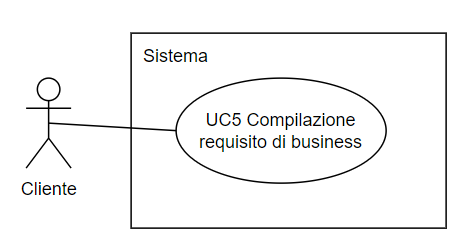
\includegraphics[width=.8\textwidth, height=.6\textheight, keepaspectratio]{documenti/imgUML/UC5-COMPILAZIONE-REQUISITO-DI-BUSINESS.png}
            \caption{UC5}
      \label{fig:UC5}
    \end{figure}
     \subsection*{Main actor}
     \begin{itemize}
         \item Cliente.
     \end{itemize}
     \subsection*{Preconditions} 
     \begin{itemize}
         \item Essere riconosciuti dal sistema come Cliente;
         \item Trovarsi nella sezione per aggiungere un nuovo requisito di business\textsubscript{G}.
     \end{itemize}
     \subsection*{Postconditions} 
        \begin{itemize}
         \item Aver compilato il campo con il requisito di business\textsubscript{G}.
        \end{itemize}
        
     \subsection*{Main scenario}

        \begin{itemize}
            \item Il cliente si trova nella pagina di compilazione dei requisiti;
            \item Il cliente compila il requisito di business\textsubscript{G}.
        \end{itemize}
    
\section{UC6-Invio requisiti di business}
    \begin{figure}[H]
      \centering
      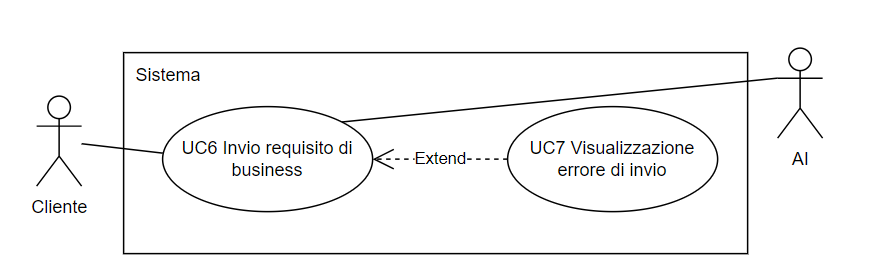
\includegraphics[width=.8\textwidth, height=.6\textheight, keepaspectratio]{documenti/imgUML/UC6-INVIO-REQUISITO-DI-BUSINESS.png}
            \caption{UC6 e UC7}
      \label{fig:UC6-INVIO-REQUISITO-DI-BUSINESS}
    \end{figure}
     \subsection*{Main actor}
     \begin{itemize}
         \item Cliente.
     \end{itemize}
      \subsection*{Second actor}
     \begin{itemize}
         \item Intelligenza Artificiale.
     \end{itemize}
     \subsection*{Preconditions} 
     \begin{itemize}
         \item Essere riconosciuti dal sistema come Cliente;
         \item Trovarsi nella sezione per aggiungere un nuovo requisito di business\textsubscript{G};
         \item Aver compilato il campo con i requisito di business\textsubscript{G}.
     \end{itemize}
     \subsection*{Postconditions} 
        \begin{itemize}
            \item Invio riuscito dei requisiti di business\textsubscript{G} all'intelligenza artificiale.
        \end{itemize}
        
     \subsection*{Main scenario}

        \begin{itemize}
            \item Invio requisito di business\textsubscript{G}.
            \item Invio requisito di business\textsubscript{G} avvenuto con successo.
        \end{itemize}
     \subsection*{Alternative scenario}
        \begin{itemize}
            \item Messaggio d'errore durante l'invio [UC7].
        \end{itemize}

\section{UC7-Errore nell'invio dei requisiti di business}

     \subsection*{Main actor}
     \begin{itemize}
         \item Cliente.
     \end{itemize}
     \subsection*{Preconditions} 
     \begin{itemize}
         \item Essere riconosciuti dal sistema come Cliente;
         \item Trovarsi nella sezione per aggiungere un nuovo requisito di business\textsubscript{G}.
     \end{itemize}
     \subsection*{Postconditions} 
        \begin{itemize}
            \item Invio dei requisiti di business\textsubscript{G} all'intelligenza artificiale non riuscito.
        \end{itemize}
        \subsection*{Main scenario}
        \begin{itemize}
        \item Invio dei requisiti di business\textsubscript{G}.
        \end{itemize}


\section{UC8-Feedback cliente sullo sviluppo user stories}
    \begin{figure}[h]
      \centering
      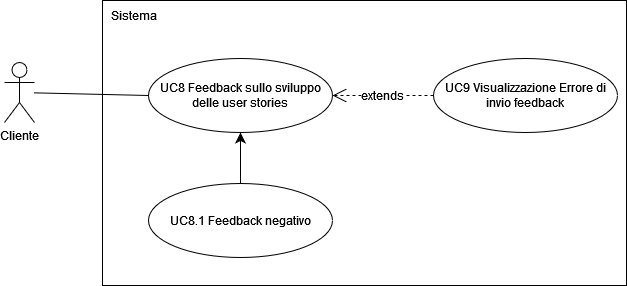
\includegraphics[width=.8\textwidth, height=.6\textheight, keepaspectratio]{documenti/imgUML/UC8-FEEDBACK-CLIENTE-SVILUPPO-USER-STORIES.drawio.png}
        \caption{UC8}
      \label{fig:UC8}
    \end{figure}
    
    \subsection*{Main actor}
    \begin{itemize}
        \item Cliente.
    \end{itemize}
    
    \subsection*{Preconditions}
    \begin{itemize}
        \item Essere riconosciuti dal sistema come Cliente;
        \item Presenza di almeno una user story\textsubscript{G}  o epic story\textsubscript{G};
        \item Epic stories completata;
        \item Trovarsi nella user story\textsubscript{G} completata nella sezione apposita per l'invio del feedback.
    \end{itemize}
    
    \subsection*{Postconditions}
    \begin{itemize}
        \item Epic/user stories completato-
    \end{itemize}
    
    \subsection*{Main scenario}
        \begin{figure}[h]
            \centering
            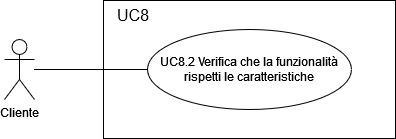
\includegraphics[width=.8\textwidth, height=.6\textheight, keepaspectratio]{documenti/imgUML/UC8-zoom.drawio.png}
            \caption{Sottocasi UC8}
            \label{fig:UC8_sottocasi}
        \end{figure}
        \begin{itemize}
            \item Verifica che la funzionalità rispetti le caratteristiche [UC8.2].
        \end{itemize}
        
    \subsection*{Alternative scenario}
    \begin{itemize}
        \item Visualizzazione errore invio feedback[UC9].
    \end{itemize}

    \subsection*{Generalize}
    \begin{figure}[h]
            \centering
            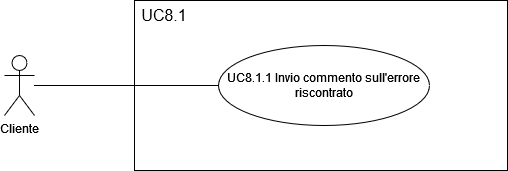
\includegraphics[width=.8\textwidth, height=.6\textheight, keepaspectratio]{documenti/imgUML/UC8.1-FEEDBACK-NEGATIVO.drawio.png}
            \caption{Generalizzazione del UC8}
            \label{fig:UC8_generalizzazione}
        \end{figure}
    \subsection{UC8.1 Feedback negativo}
    \begin{itemize}
            \item Invio commento sull'errore riscontrato [UC8.1.1].
        \end{itemize}
    \newpage
        
\section{UC9-Errore nell'invio del feedback}

     \subsection*{Main actor}
     \begin{itemize}
         \item Cliente.
     \end{itemize}
     \subsection*{Preconditions} 
 \begin{itemize}
        \item Essere riconosciuti dal sistema come Cliente;
        \item Presenza di almeno una user story\textsubscript{G}  o epic story\textsubscript{G};
        \item Epic stories\textsubscript{G}  completata;
        \item Trovarsi nella user story\textsubscript{G}  completata nella sezione apposita per l'invio del feedback.
    \end{itemize}
     \subsection*{Postconditions} 
        \begin{itemize}
            \item Invio del feedback al Project Manager\textsubscript{G}  non riuscito.
        \end{itemize} 
        \subsection*{Main scenario}
        \begin{itemize}
            \item Invio del feedback al Project Manager\textsubscript{G}.
        \end{itemize}

        
\section{UC10- Validazione finale del feedback}

\begin{figure}[h]
      \centering
      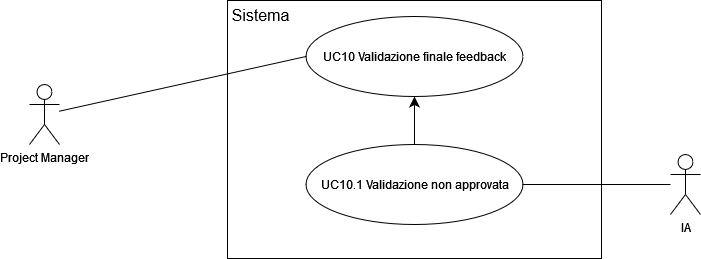
\includegraphics[width=.8\textwidth, height=.6\textheight, keepaspectratio]{documenti/imgUML/UC10-VALIDAZIONE-FINALE-FEEDBACK.drawio.png}
        \caption{UC10}
      \label{fig:UC10}
    \end{figure}
    
    \subsection*{Main actor}
    \begin{itemize}
        \item Project Manager\textsubscript{G}.
    \end{itemize}
    
    \subsection*{Preconditions}
    \begin{itemize}
        \item Aver ricevuto dal Cliente un feedback negativo riguardante il lavoro finito;
        \item Presenza di almeno una user story\textsubscript{G}  o epic story\textsubscript{G};
        \item Epic stories\textsubscript{G}  completata.
    \end{itemize}
    
    \subsection*{Postconditions}
    \begin{itemize}
        \item Epic/user stories\textsubscript{G}  completato;
        \item Feedback per epic/user stories\textsubscript{G}  ricevuto dal sistema.
    \end{itemize}
    
    \subsection*{Main scenario}
        \begin{figure}[h]
            \centering
            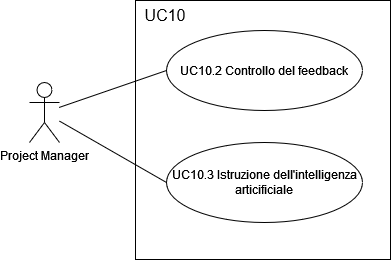
\includegraphics[width=.8\textwidth, height=.6\textheight, keepaspectratio]{documenti/imgUML/UC10-zoom.drawio.png}
            \caption{Sottocasi UC10}
            \label{fig:UC10_sottocasi}
        \end{figure}
        \begin{itemize}
            \item Controllo del feedback inviato [UC10.2];
            \item Istruzione dell'intelligenza artificiale [UC10.3].
        \end{itemize}
        
    \subsection*{Generalize}
      \begin{figure}[h]
            \centering
            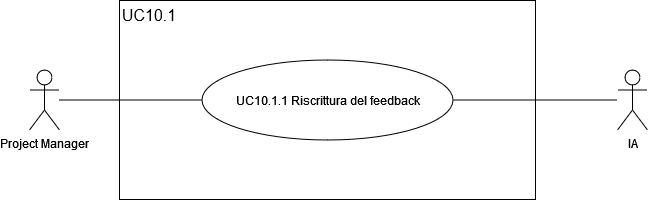
\includegraphics[width=.8\textwidth, height=.6\textheight, keepaspectratio]{documenti/imgUML/UC10.1-VALIDAZIONE-FEEDBACK-NON-APPROVATA.drawio.png}
            \caption{Generalizzazione del UC10}
            \label{fig:UC10_generalizzazione}
        \end{figure}
    \subsection{UC10.1 Validazione del feedback non approvata}
    \begin{itemize}
        \item Riscrittura del feedback da parte del Project Manager\textsubscript{G}  [UC10.1.1].
        \subsection*{UC10.1.1 Riscrittura del feedback da parte del Project Manager\textsubscript{G} }
     \subsection*{Main actor}
         \begin{itemize}
             \item Project Manager\textsubscript{G}.
         \end{itemize}
     \subsection*{Preconditions} 
        \begin{itemize}
            \item Aver ricevuto un feedback negativo dal cliente;
            \item Il feedback non è comprensibile dall'intelligenza artificiale.
        \end{itemize}
        \subsection*{Postcondition} 
        \begin{itemize}
            \item Il feedback è scritto in modo comprensibile dall'intelligenza artificiale.
        \end{itemize}
        \subsection*{Main scenario}
        \begin{itemize}
        \item Il Project Manager\textsubscript{G} riscrive il feedback del cliente.
        \end{itemize}
    \end{itemize}
    
\subsection{UC10.2-Controllo del feedback inviato}
    
     \subsection*{Main actor}
         \begin{itemize}
             \item Cliente.
         \end{itemize}
     \subsection*{Preconditions} 
        \begin{itemize}
            \item Aver ricevuto un feedback negativo dal cliente.
        \end{itemize}
        \subsection*{Postcondition} 
        \begin{itemize}
            \item Il feedback è scritto in modo comprensibile per intelligenza artificiale.
        \end{itemize}
        \subsection*{Main scenario}
        \begin{itemize}
            \item Il Project Manager\textsubscript{G} riscrive il feedback.
        \end{itemize}

    \subsection{UC10.3-Istruzione dell'intelligenza artificiale}
     \subsection*{Main actor}
         \begin{itemize}
             \item Cliente.
         \end{itemize}
     \subsection*{Preconditions} 
        \begin{itemize}
            \item Avere un feedback scritto in modo comprensibile dal cliente.
        \end{itemize}
        \subsection*{Main scenario}
        \begin{itemize}
            \item L'intelligenza artificiale elabora il feedback.
        \end{itemize}
        \subsection*{Postcondition} 
        \begin{itemize}
            \item L'intelligenza artificiale è stata istruita grazie al feedback ricevuto.
        \end{itemize}
        

\section{UC11-Visualizzazione andamento progetto}
    \begin{figure}[h]
      \centering
      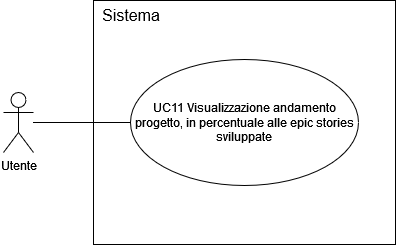
\includegraphics[width=.8\textwidth, height=.6\textheight, keepaspectratio]{documenti/imgUML/UC11-VISUALIZZAZIONE-ANDAMENTO-PROGETTO.drawio.png}
        \caption{UC11}
      \label{fig:UC11}
    \end{figure}
    
    \subsection*{Main actor}
        \begin{itemize}
            \item Utente.
        \end{itemize}
        
    \subsection*{Preconditions}
        \begin{itemize}
            \item Essere riconosciuti dal sistema con i propri privilegi;
            \item Cliente ha inviato con successo i requisiti di business\textsubscript{G} al sistema;
            \item Requisiti di business\textsubscript{G} sono stati elaborati dal sistema;
            \item Project Manager\textsubscript{G} ha accettato le epic/user stories\textsubscript{G} generate dal sistema;
            \item Project Manager\textsubscript{G} ha assegnato le epic/user stories\textsubscript{G} agli Sviluppatori.
        \end{itemize}
        
    \subsection*{Postconditions}
        \begin{itemize}
            \item Presa visione dell'andamento del progetto.
        \end{itemize}
        
    \subsection*{Main scenario}
        
        \begin{itemize}
            \item Visualizzazione della percentuale rappresentante il quantitativo di epic/user stories\textsubscript{G} sviluppate.
        \end{itemize}
        

\section{UC12-Feedback epic/user stories\textsubscript{G} Project Manager\textsubscript{G}}
    \begin{figure}[h]
      \centering
      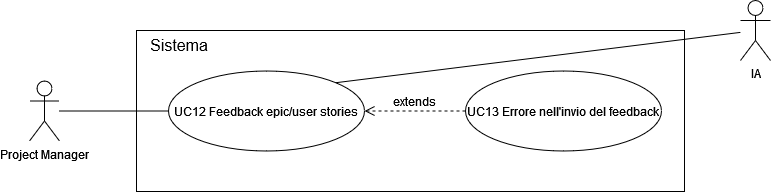
\includegraphics[width=.8\textwidth, height=.6\textheight, keepaspectratio]{documenti/imgUML/UC12-FEEDBACK-EPIC-USER-STORIES-PROJECT-MANAGER.drawio.png}
    \caption{UC12}      
      \label{fig:UC12}
    \end{figure}
%con feedback si intende un effetto di reazione prodotto da un messaggio su chi lo ha emesso
    \subsection*{Main actor}
    \begin{itemize}
        \item Project Manager\textsubscript{G}.
    \end{itemize}
    \subsection*{Second actor}
    \begin{itemize}
        \item Intelligenza artificiale.
    \end{itemize}
    
    \subsection*{Preconditions}
        \begin{itemize}
            \item Essere riconosciuti dal sistema come Project Manager\textsubscript{G};
            \item Cliente ha inviato con successo i requisiti di business\textsubscript{G} al sistema;
            \item Requisiti di business\textsubscript{G} sono stati elaborati dal sistema.
        \end{itemize}
        
    \subsection*{Postconditions}
        \begin{itemize}
            \item Feedback per epic/user stories ricevuto dal sistema;
            \item Il sistema ha generato epic/user stories\textsubscript{G} corrette, con corrispettivo tag\textsubscript{G}.
        \end{itemize}
        
    \subsection*{Main scenario}
        \begin{figure}[h]
          \centering
          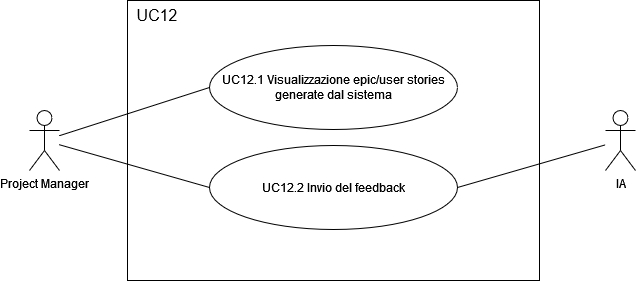
\includegraphics[width=.8\textwidth, height=.6\textheight, keepaspectratio]{documenti/imgUML/UC12-zoom.drawio.png}
          \caption{Sottocasi UC12}
          \label{fig:UC12_sottocasi}
        \end{figure}

        \begin{itemize}
            \item Project Manager\textsubscript{G} visualizza epic/user stories\textsubscript{G} generate dal sistema [UC12.1];
            \item Project Manager\textsubscript{G} invia il feedback al sistema [UC12.2].
        \end{itemize}
        
    \subsection*{Alternative scenario}
        
        \begin{itemize}
            \item Errore nell'invio del feedback[UC13];
        \end{itemize}
        
\section{UC13-Errore nell'invio del feedback}

     \subsection*{Main actor}
     \begin{itemize}
         \item Project Manager\textsubscript{G}.
     \end{itemize}
   \subsection*{Preconditions}
        \begin{itemize}
            \item Essere riconosciuti dal sistema come Project Manager\textsubscript{G};
            \item Cliente ha inviato con successo i requisiti di business\textsubscript{G} al sistema;
            \item Requisiti di business\textsubscript{G} sono stati elaborati dal sistema.
        \end{itemize}
        
    \subsection*{Postconditions}
        \begin{itemize}
            \item Feedback per epic/user stories\textsubscript{G} non inviato al sistema;
            \item Visualizzazione del messaggio di errore di invio.
        \end{itemize} 
        \subsection*{Main scenario}
        \begin{itemize}
            \item Il Project Manager\textsubscript{G} invia il feedback al sistema.
        \end{itemize}

  
\section{UC14-Visualizzazione personalizzata epic/user stories\textsubscript{G}}
    \begin{figure}[h]
      \centering
      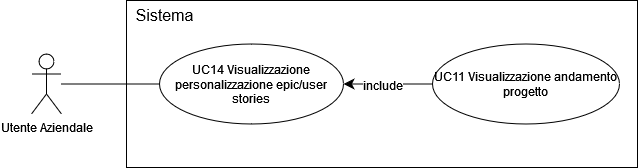
\includegraphics[width=.8\textwidth, height=.6\textheight, keepaspectratio]{documenti/imgUML/UC14-VISUALIZZAZIONE-PERSONALIZZATA-EPIC-USER-STORIES.drawio.png}
        \caption{UC14}
      \label{fig:UC14}
    \end{figure}
    
    \subsection*{Main actor}
        \begin{itemize}
            \item Utente Aziendale.
        \end{itemize}
        
    \subsection*{Preconditions}
        \begin{itemize}
            \item Essere riconosciuti dal sistema con i propri permessi;
            \item Cliente ha inviato con successo i requisiti di business\textsubscript{G} al sistema;
            \item requisiti di business\textsubscript{G} sono stati elaborati dal sistema;
            \item Project Manager\textsubscript{G} ha accettato le epic/user stories\textsubscript{G} generate dal sistema;
            \item Project Manager\textsubscript{G} ha assegnato le epic/user stories\textsubscript{G} agli Sviluppatori.
        \end{itemize}
        
    \subsection*{Postconditions}
    \begin{itemize}
        \item Project Manager\textsubscript{G} ha preso visione dell'andamento del progetto.
    \end{itemize}
    
    \subsection*{Main scenario}
        \begin{itemize}
            \item Project Manager\textsubscript{G} visualizza la lista delle epis/user stories\textsubscript{G} assegnate.
        \end{itemize}
        
    \subsection*{Inclusione}
        \begin{itemize}
            \item Visualizzazione andamento progetto [UC11].
        \end{itemize}

\section{UC15-Assegnazione epic/user stories \textsubscript{G}}
    \begin{figure}[h]
      \centering
      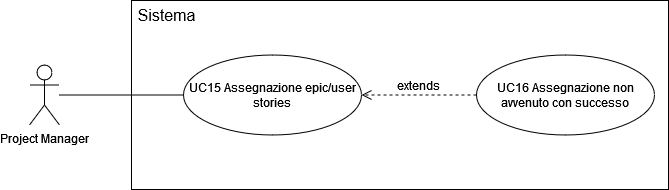
\includegraphics[width=.8\textwidth, height=.6\textheight, keepaspectratio]{documenti/imgUML/UC15-ASSEGNAZIONE-EPIC-USER-STORIES.drawio.png}
    \caption{UC15}
      \label{fig:UC15}
    \end{figure}

    \subsection*{Main actor}
    \begin{itemize}
        \item Project Manager\textsubscript{G}.
    \end{itemize}
    
    \subsection*{Preconditions}
        \begin{itemize}
            \item Essere riconosciuto dal sistema come Project Manager\textsubscript{G};
            \item Le epic/user stories\textsubscript{G} che si vogliono assegnare devono avere feedback positivo;
            \item Trovarsi nella pagina della epic story\textsubscript{G} da assegnare.
        \end{itemize}
        
    \subsection*{Postconditions}
        \begin{itemize}
            \item Una o più epic/user stories\textsubscript{G} con feedback positivo è stata assegnata ad uno o più Sviluppatori.
        \end{itemize}
    
    \subsection*{Main scenario}
        \begin{figure}[h]
          \centering
          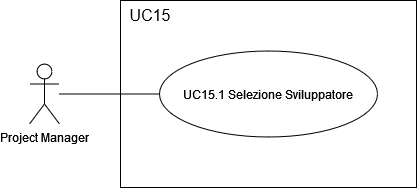
\includegraphics[width=.8\textwidth, height=.6\textheight, keepaspectratio]{documenti/imgUML/UC15-zoom.drawio.png}
          \caption{Sottocasi UC15}
          \label{fig:UC15_sottocasi}
        \end{figure}
        
        \begin{itemize}
            \item Project Manager\textsubscript{G} seleziona lo Sviluppatore a cui assegnare la epic/user stories\textsubscript{G} selezionata [UC15.1].
        \end{itemize}
        
    \subsection*{Alternative scenario}
        \begin{itemize}
            \item Errore nell'assegnazione dell'epic story\textsubscript{G} [UC16].
        \end{itemize}    
        
    \subsection{UC15.1- Selezione dello sviluppatore}
        \subsection*{Main actor}
    \begin{itemize}
        \item Project Manager\textsubscript{G}.
    \end{itemize}
    
    \subsection*{Preconditions}
        \begin{itemize}
            \item Essere riconosciuto dal sistema come Project Manager\textsubscript{G};
            \item Le epic/user stories\textsubscript{G} che si vogliono assegnare devono avere feedback positivo;
            \item Trovarsi nella pagina della epic story\textsubscript{G} da assegnare.
        \end{itemize}
        
    \subsection*{Postconditions}
        \begin{itemize}
            \item Una o più epic/user stories\textsubscript{G} con feedback positivo è stata assegnata ad uno o più Sviluppatori.
        \end{itemize}

    \subsection*{Main scenario}
    \begin{itemize}
        \item Il Project Manager\textsubscript{G} seleziona a quale o quali sviluppatori assegnare le epic/user stories\textsubscript{G}.
    \end{itemize}

\section{UC16 Assegnazione non avvenuta}

       \subsection*{Main actor}
    \begin{itemize}
        \item Project Manager\textsubscript{G}.
    \end{itemize}
    
    \subsection*{Preconditions}
        \begin{itemize}
            \item Essere riconosciuto dal sistema come Project Manager\textsubscript{G};
            \item Le epic/user stories\textsubscript{G} che si vogliono assegnare devono avere feedback positivo;
            \item Trovarsi nella pagina della epic story\textsubscript{G} da assegnare.
        \end{itemize}
        
    \subsection*{Postconditions}
        \begin{itemize}
            \item L'assegnazione non è avvenuta con successo.
            \item Visualizzazione del messaggio di errore di assegnazione.
        \end{itemize}

    \subsection*{Main scenario}
    \begin{itemize}
        \item Il Project Manager\textsubscript{G} seleziona a quale o quali sviluppatori assegnare le epic/user stories\textsubscript{G}.
    \end{itemize}

\section{UC17 Inserimento del Tag\textsubscript{G}}
\subsection*{Main actor}
        \begin{itemize}
            \item Sviluppatore.
        \end{itemize}
    
    \subsection*{Preconditions}
        \begin{itemize}
            \item Essere riconosciuti dal sistema come Sviluppatore;
            \item Avere un'assegnazione per quella user story\textsubscript{G} dal Project Manager\textsubscript{G}.
        \end{itemize}
        
    \subsection*{Postconditions} 
        \begin{itemize}
            \item Il codice è correttamente taggato\textsubscript{G}.
        \end{itemize}

    \subsection*{Main scenario}
        \begin{itemize}
            \item Inserimento tag\textsubscript{G} di apertura per invio codice.
            \item Inserimento tag\textsubscript{G} di chiusura per invio codice.
        \end{itemize}

        
        
\section{UC18 Verifica codice da parte dell'IA\textsubscript{G}}
    \begin{figure}[h]
      \centering
      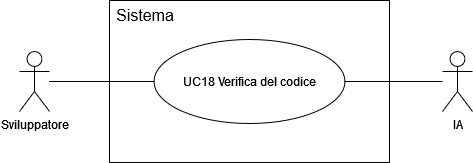
\includegraphics[width=.8\textwidth, height=.6\textheight, keepaspectratio]{documenti/imgUML/UC18-VERIFICA-CODICE-IA.drawio.png}
        \caption{UC18}
      \label{fig:UC18}
    \end{figure}
    
    \subsection*{Main actor}
        \begin{itemize}
            \item Sviluppatore.
        \end{itemize}
    \subsection*{Second actor}
        \begin{itemize}
            \item Intelligenza Artificiale.
        \end{itemize}
    
    \subsection*{Preconditions}
        \begin{itemize}
            \item Essere riconosciuti dal sistema come Sviluppatore;
            \item Cliente ha inviato requisiti di business\textsubscript{G};
            \item Project Manager\textsubscript{G} ha accettato epic/user stories\textsubscript{G};
            \item Project Manager\textsubscript{G} ha assegnato epic/user stories\textsubscript{G};
            \item Sviluppatore ha sviluppato codice e test\textsubscript{G} riguardante una o più user story\textsubscript{G};
            \item Sviluppatore ha taggato\textsubscript{G} correttamente il codice.
        \end{itemize}
        
    \subsection*{Postconditions}
        \begin{itemize}
            \item Sviluppatore riceve feedback da parte del sistema riguardante il codice inviato.
        \end{itemize}
    
    \subsection*{Main scenario}
        \begin{figure}[h]
          \centering
          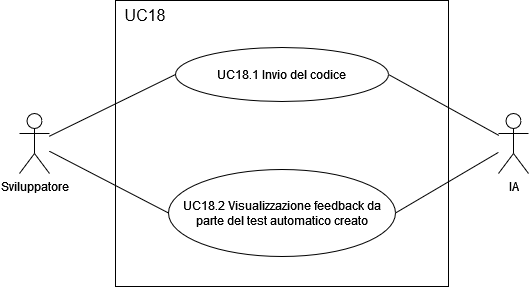
\includegraphics[width=.8\textwidth, height=.6\textheight, keepaspectratio]{documenti/imgUML/UC18-zoom.drawio.png}
          \caption{Sottocasi UC18}
          \label{fig:UC18_sottocasi}
        \end{figure}
        
        \begin{itemize}
            \item Sviluppatore invia codice per la verifica [UC18.1];

            \item Sviluppatore riceve feedback dal sistema riguardante il codice inviato [UC18.2].
        \end{itemize}
        
    \subsection{UC18.1- Invio codice per la verifica}
    \subsection*{Main actor}
        \begin{itemize}
            \item Sviluppatore.
        \end{itemize}
        
    \subsection*{Preconditions}
        \begin{itemize}
            \item Essere riconosciuti dal sistema come Sviluppatore;
            \item Cliente ha inviato requisiti di business\textsubscript{G};
            \item Project Manager\textsubscript{G} ha accettato epic/user stories\textsubscript{G};
            \item Project Manager\textsubscript{G} ha assegnato epic/user stories\textsubscript{G};
            \item Sviluppatore ha sviluppato codice e test\textsubscript{G} riguardante una o più user story\textsubscript{G};
            \item Sviluppatore ha taggato\textsubscript{G} correttamente il codice.
        \end{itemize}

    \subsection*{Postconditions}
        \begin{itemize}
            \item Invio del codice al sistema avvenuto con successo.
        \end{itemize}

    \subsection*{Main scenario}
        \begin{itemize}
            \item Sviluppatore invia codice taggato al sistema.
        \end{itemize}
        
    \subsection{UC18.2- Visualizzazione feedback}
    \subsection*{Main actor}
        \begin{itemize}
            \item Sviluppatore.
        \end{itemize}
        
    \subsection*{Preconditions}
        \begin{itemize}
            \item Essere riconosciuti dal sistema come Sviluppatore;
            \item Cliente ha inviato requisiti di business\textsubscript{G};
            \item Project Manager\textsubscript{G} ha accettato epic/user stories\textsubscript{G};
            \item Project Manager\textsubscript{G} ha assegnato epic/user stories\textsubscript{G};
            \item Sviluppatore ha sviluppato codice e test\textsubscript{G} riguardante una o più user story\textsubscript{G};
            \item Sviluppatore ha taggato\textsubscript{G} correttamente il codice.
        \end{itemize}
        
    \subsection*{Postconditions}
        \begin{itemize}
            \item Sviluppatore riceve feedback da parte del sistema riguardante il codice inviato;
            \item Il codice può essere sistemato, in base a quello consigliato dall'intelligenza artificiale.
        \end{itemize}

    \subsection*{Main scenario}
        \begin{itemize}
            \item Sviluppatore visualizza feedback del sistema.
        \end{itemize}
    

        
\section{UC19 Inserimento di un nuovo cliente}
    \begin{figure}[h]
      \centering
      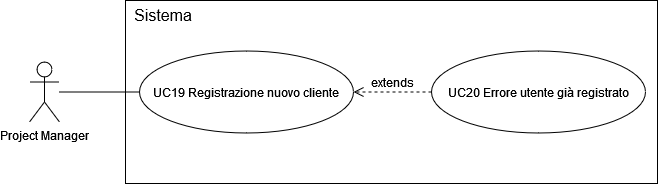
\includegraphics[width=.8\textwidth, height=.6\textheight, keepaspectratio]{documenti/imgUML/UC19-INSERIMENTO-NUOVO-CLIENTE.drawio.png}
    \caption{UC19}
      \label{fig:UC19}
    \end{figure}
    
    \subsection*{Main actor}
        \begin{itemize}
            \item Project Manager\textsubscript{G}.
        \end{itemize}
        
    \subsection*{Preconditions}
        \begin{itemize}
            \item Essere riconosciuti dal sistema come Project Manager\textsubscript{G};
            \item Cliente ha preso contatto con l'azienda per l'inizio di un nuovo progetto insieme.
        \end{itemize}
        
    \subsection*{Postconditions}
        \begin{itemize}
            \item Cliente registrato nel sistema;
            \item Cliente può effettuare il primo accesso.
        \end{itemize}
    
    \subsection*{Main scenario}
        \begin{figure}[h]
          \centering
          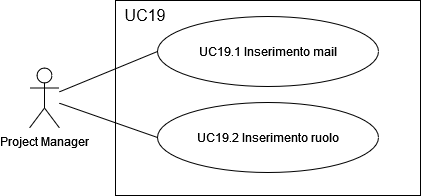
\includegraphics[width=.8\textwidth, height=.6\textheight, keepaspectratio]{documenti/imgUML/UC19-zoom.drawio.png}
          \caption{Sottocasi UC19}
          \label{fig:UC19_sottocasi}
        \end{figure}
        
        \begin{itemize}
            \item Il Project Manager\textsubscript{G} inserisce mail [UC19.1];
            \item Il Project Manager\textsubscript{G} inserisce ruolo di Cliente [UC19.2].
        \end{itemize}
        
    \subsection*{Alternative scenario}
        \begin{itemize}
            \item Errore nella registrazione dell'utente [UC20].
        \end{itemize}

    \subsection{UC19.1- Inserimento Mail}
    \subsection*{Main actor}
        \begin{itemize}
            \item Project Manager\textsubscript{G}.
        \end{itemize}
        
    \subsection*{Preconditions}
        \begin{itemize}
            \item Essere riconosciuti dal sistema come Project Manager\textsubscript{G};
            \item Cliente ha preso contatto con l'azienda per l'inizio di un nuovo progetto insieme.
        \end{itemize}
    
    \subsection*{Postconditions}
        \begin{itemize}
            \item La mail è stata inserita con successo.
        \end{itemize}

    \subsection*{Main scenario}
        \begin{itemize}
            \item Inserimento mail nel campo "mail".
        \end{itemize}
        

    \subsection{UC19.2- Inserimento ruolo}
    \subsection*{Main actor}
        \begin{itemize}
            \item Project Manager\textsubscript{G}.
        \end{itemize}
        
    \subsection*{Preconditions}
        \begin{itemize}
            \item Essere riconosciuti dal sistema come Project Manager\textsubscript{G};
            \item Cliente ha preso contatto con l'azienda per l'inizio di un nuovo progetto insieme.
        \end{itemize}
        
    \subsection*{Postconditions}
        \begin{itemize}
            \item Cliente registrato nel sistema;
            \item Cliente può effettuare il primo accesso.
        \end{itemize}

    \subsection*{Main scenario}
        \begin{itemize}
            \item inserimento ruolo nel campo "ruolo".
        \end{itemize}

\section{UC20- Errore nella registrazione dell'utente}
\subsection*{Main actor}
        \begin{itemize}
            \item Project Manager\textsubscript{G}.
        \end{itemize}
        
    \subsection*{Preconditions}
        \begin{itemize}
            \item Essere riconosciuti dal sistema come Project Manager\textsubscript{G};
            \item Cliente ha preso contatto con l'azienda per l'inizio di un nuovo progetto insieme.
        \end{itemize}
        
    \subsection*{Postconditions}
        \begin{itemize}
            \item Messaggio di errore nella registrazione del nuovo utente cliente.
        \end{itemize}

    \subsection*{Main scenario}
        \begin{itemize}
            \item Compilazione dati cliente.
            \item Invio dati cliente.
        \end{itemize}
\section{UC21 Primo accesso}
 \begin{figure}[h]
          \centering
          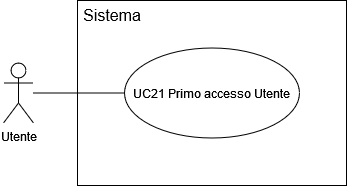
\includegraphics[width=.8\textwidth, height=.6\textheight, keepaspectratio]{documenti/imgUML/UC21-PRIMO-ACCESSO.drawio.png}
            \caption{UC21}
          \label{fig:UC21}
        \end{figure}
\subsection*{Main actor}
        \begin{itemize}
            \item Utente.
        \end{itemize}
        
    \subsection*{Preconditions}
        \begin{itemize}
            \item Essere riconosciuti dal sistema con il proprio ruolo;
            \item Non aver ancora effettuato il primo accesso.
        \end{itemize}
        
    \subsection*{Postconditions}
        \begin{itemize}
            \item Cliente registrato nel sistema con la nuova password;
            \item Cliente può iniziare a scrivere i suoi requisisti di business\textsubscript{G}.
        \end{itemize}

        \subsection*{Main scenario}
        \begin{figure}[h]
          \centering
          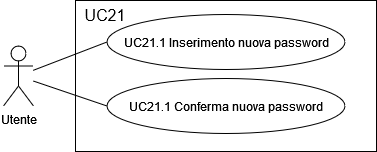
\includegraphics[width=.8\textwidth, height=.6\textheight, keepaspectratio]{documenti/imgUML/UC21-zoom.drawio.png}
            \caption{Sottocasi UC21}
          \label{fig:UC21_sottocasi}
        \end{figure}
        
        \begin{itemize}
            \item Inserimento nuova password [UC21.1];
            \item Conferma nuova password [UC21.2].
        \end{itemize}
     

        \subsection{UC21.1 Inserimento nuova password}
            \subsection*{Main actor}
        \begin{itemize}
            \item Utente.
        \end{itemize}
        
    \subsection*{Preconditions}
        \begin{itemize}
            \item Essere riconosciuti dal sistema con il proprio ruolo;
            \item Non aver ancora effettuato il primo accesso.
        \end{itemize}

    \subsection*{Postconditions}
        \begin{itemize}
            \item Nuova password inserita.
        \end{itemize}

        \subsection*{Main scenario}
        \begin{itemize}
            \item Scrivere nuova password nel campo "nuova password".
        \end{itemize}

    \subsection{UC21.2- Conferma nuova password}
    \subsection*{Main actor}
        \begin{itemize}
            \item Utente.
        \end{itemize}
        
    \subsection*{Preconditions}
        \begin{itemize}
            \item Essere riconosciuti dal sistema con il proprio ruolo;
            \item Non aver ancora effettuato il primo accesso.
            \item Aver inserito la nuova password.
        \end{itemize}
        
    \subsection*{Postconditions}
        \begin{itemize}
            \item Cliente registrato nel sistema con la nuova password;
            \item Cliente può iniziare a scrivere i suoi requisisti di business\textsubscript{G}.
        \end{itemize}

    \subsection*{Main scenario}
        \begin{itemize}
            \item Conferma nuova password inserita.
        \end{itemize}

\newpage
\section{Requisiti}
\subsection{Requisiti funzionali}
\begin{center}
    \begin{tabular}{|p{2cm}|p{3cm}|p{6cm}|p{3cm}|p{2cm}|}
    \rowcolor{Blue} 
\hline
ID & Classificazione & Descrizione & Indirizzato a&Casi d'uso\textsubscript{G}  \\ 
\rowcolor{LightBlue}
\hline
ROF1&Obbligatorio & Accesso a web app\textsubscript{G} tramite login composto da email e password. & utente registrato ma non ancora riconosciuto dal sistema & UC1, UC16, UC18 \\ 
\rowcolor{LighterBlue}
\hline
ROF2&Obbligatorio & Scrittura di richieste di business\textsubscript{G} tramite box testuale da web app\textsubscript{G}. & Cliente & UC3\\ 
\rowcolor{LightBlue}
\hline
ROF3&Obbligatorio & Invio delle richieste di business\textsubscript{G} da web app. \textsubscript{G} & Cliente & UC3\\
\hline
\rowcolor{LighterBlue}

ROF4&Obbligatorio & Visualizzazione andamento sviluppo richieste tramite barra di completamento basata sulla percentuale di user stories\textsubscript{G} completate. & Cliente, Project Manager\textsubscript{G} & UC8, UC11\\
\rowcolor{LightBlue}
\hline
ROF5&Obbligatorio & Approvazione o rifiuto del risultato relativo all'implementazione di una user story\textsubscript{G}. & Cliente & UC5\\
\hline
\rowcolor{LighterBlue}

RDF6&Desiderabile & Ricezione notifiche quando user story\textsubscript{G} completata. & Cliente & UC5 UC8\\
\hline
\rowcolor{LightBlue}
\hline
ROF7&Obbligatorio & Funzionalità di tag\textsubscript{G} nel plug-in\textsubscript{G}.  & Sviluppatore & UC14\\
\hline
\rowcolor{LighterBlue}

ROF8&Obbligatorio & Lista di user stories\textsubscript{G} assegnate da Project Manager\textsubscript{G} sia su web app\textsubscript{G} che su plug-in\textsubscript{G}. & Sviluppatore & UC14 UC15\\
\hline
\rowcolor{LightBlue}

RDF9&Desiderabile & Ricezione notifica su web app\textsubscript{G} quando nuova user story\textsubscript{G} è assegnata dal Project Manager\textsubscript{G}.& Sviluppatore & UC12\\
\hline
\rowcolor{LighterBlue}
ROF10&Obbligatorio & Invio del codice sviluppato a IA\textsubscript{G} per richiesta verifica.& Sviluppatore & UC15\\

\hline
\end{tabular}

    \begin{tabular}{|p{2cm}|p{3cm}|p{6cm}|p{3cm}|p{2cm}|}
    \rowcolor{Blue} 
\hline
ID & Classificazione & Descrizione & Indirizzato a&Casi d'uso\textsubscript{G}  \\ 
\rowcolor{LighterBlue}

ROF11&Obbligatorio & Visualizzazione user stories\textsubscript{G} generate da IA\textsubscript{G}.  & Project Manager\textsubscript{G} & UC9\\
\hline



\rowcolor{LightBlue}
\hline
ROF12&Obbligatorio & Invio di feedback sulle user stories\textsubscript{G} generate all'IA\textsubscript{G}.& Project Manager\textsubscript{G}&UC9\\
\hline
\rowcolor{LighterBlue}

ROF13&Obbligatorio & Suddivisione delle user stories\textsubscript{G} troppo grandi.  & Project Manager\textsubscript{G}& UC9\\
\hline

\rowcolor{LightBlue}

ROF14&Obbligatorio & Assegnazione user stories\textsubscript{G} agli sviluppatori.& Project Manager\textsubscript{G}& UC12\\
\hline

\rowcolor{LighterBlue}

RDF15&Desiderabile & Ricezione notifiche quando user story\textsubscript{G} viene generata in seguito a richiesta del cliente. & Project Manager\textsubscript{G} & UC7\\
\hline

\rowcolor{LightBlue}

ROF16&Obbligatorio & Invio richiesta di modifiche relative a user stories\textsubscript{G} a IA\textsubscript{G} prima di approvazione. & Project Manager\textsubscript{G}& UC7\\
\hline
\rowcolor{LighterBlue}

ROF17&Obbligatorio & Visualizzazione andamento epic/user stories\textsubscript{G} assegnate.& Sviluppatore& UC11\\

\hline

\rowcolor{LightBlue}
ROF18&Obbligatorio & Creazione di un plug-in\textsubscript{G} per VSCode\textsubscript{G}.& Project Manager\textsubscript{G}, Sviluppatore& UC14, UC15\\
\hline
\rowcolor{LighterBlue}
RDF19&Desiderabile & Creazione di un plug-in\textsubscript{G} per XCode\textsubscript{G}.& Project Manager\textsubscript{G}, Sviluppatore& UC14, UC15\\
\hline
\rowcolor{LightBlue}
ROF20&Obbligatorio & I linguaggi supportati dal plug-in sono Typescript\textsubscript{G} e Javascript\textsubscript{G}. & Project Manager\textsubscript{G}, Sviluppatore &UC14, UC15\\
\hline
\rowcolor{LighterBlue}
RDF21&Desiderabile & Altri linguaggi che potrebbero essere supportati in futuro sono Kotlin\textsubscript{G} e Swift\textsubscript{G}.& Project Manager\textsubscript{G}, Sviluppatore &UC14, UC15\\
\hline
\rowcolor{LightBlue}
ROF22 & Obbligatorio & Gestione degli input (prevenzione da Injection\textsubscript{G} Cross Site Scripting\textsubscript{G} e sanificazione dell'input.) & Cliente, Project Manager\textsubscript{G}, Sviluppatore & \\
\hline

\end{tabular}
\captionof{table}{Tabella dei requisiti funzionali}
\label{tab:reqfunz}
\end{center}

\subsection{Requisiti di qualità}

\begin{center}
    \begin{tabular}{|p{3cm}|p{3cm}|p{6cm}|}
    \rowcolor{Blue} 
\hline
ID & Classificazione & Descrizione\\ 
\rowcolor{LightBlue}
\hline
ROQ1& Obbligatorio & Il progetto deve essere accessibile pubblicamente su GitHub\textsubscript{G} o su un'altra repository\textsubscript{G} pubblica.\\ 
\rowcolor{LighterBlue}
\hline
ROQ2& Obbligatorio & Il prodotto deve essere sviluppato conformemente a quanto stabilito nelle \textit{Norme Way of Working\textsubscript{G}}. \\ 
\rowcolor{LightBlue}
\hline
ROQ3& Obbligatorio & Deve essere effettuato il testing\textsubscript{G} delle unità e dell'integrazione con una copertura minima dell'80\%.\\
\hline
\rowcolor{LighterBlue}

ROQ4& Obbligatorio & Deve essere fornita una documentazione completa sulle scelte implementative e progettuali effettuate.\\
\hline
\rowcolor{LightBlue}
ROQ5& Obbligatorio & Deve essere fornito un manuale per l'utilizzo del prodotto.\\
\hline
\rowcolor{LighterBlue}
ROQ6& Obbligatorio & Deve essere fornita una documentazione che compara la capacità di ChatGPT\textsubscript{G} e quella di AWS Bedrock\textsubscript{G} nell'interpretare del codice sorgente ed associare le user stories\textsubscript{G} generate.\\
\hline
\rowcolor{LightBlue}
ROQ7& Obbligatorio & Deve essere fornita una documentazione che prova un'interpretazione corretta da parte dell'IA\textsubscript{G} che si basa: sulle epic/user stories\textsubscript{G} generate dall'IA\textsubscript{G}, i test generati dall'IA\textsubscript{G}, i criteri di accettazione delle epic/user stories\textsubscript{G} forniti dal proponente.\\
\hline
\end{tabular}
\captionof{table}{Tabella dei requisiti di quailità}
\label{tab:reqal}
\end{center}
\newpage



\subsection{Requisiti di vincolo}
Di seguito la specifica per i requisiti di vincolo, i quali descrivono i limiti e le restrizioni che un sistema
deve rispettare per soddisfare le esigenze dell'utente.
\begin{center}

    \begin{tabular}{|p{3cm}|p{3cm}|p{6cm}|}
    \rowcolor{Blue} 
\hline
ID & Classificazione & Descrizione \\ 
\rowcolor{LightBlue}
\hline
ROV1& Obbligatorio & L'applicazione per l'interazione con la piattaforma dev'essere sviluppata attraverso l'uso di tecnologie web.\\ 
\hline
\rowcolor{LighterBlue}
ROV2& Obbligatorio & Le due IA\textsubscript{G} utilizzate per l'analisi sono AWS Bedrock\textsubscript{G} e ChatGPT\textsubscript{G}. \\ 
\rowcolor{LightBlue}
\hline
RDV3& Desiderabile & L'applicazione deve essere utilizzabile tramite browser (Chrome 123.0, Firefox 124.0, Safari 17.0) di dispositivi mobili(Android 14.0, iOS 17.0).\\
\hline
\rowcolor{LighterBlue}

ROV4& Obbligatorio & Il front-end\textsubscript{G} dell'applicazione verrà sviluppato in React\textsubscript{G}.\\
\rowcolor{LightBlue}
\hline
ROV5& Obbligatorio & Ogni AWS Lambda-function\textsubscript{G} deve essere sviluppata in Node.js\textsubscript{G}.\\
\hline
\rowcolor{LighterBlue}

ROV6& Obbligatorio & Tutte le API\textsubscript{G} devono essere integrate in AWS API-gateway\textsubscript{G}.\\
\hline
\rowcolor{LightBlue}
ROV7& Obbligatorio & L'applicativo deve essere compatibile con il browser Google Chrome\textsubscript{G} dalla versione\textsubscript{G} 121.\\
\hline
\rowcolor{LighterBlue}
ROV8& Obbligatorio & L'applicativo deve essere compatibile con il browser Firefox\textsubscript{G} dalla versione\textsubscript{G} 122.\\
\hline
\end{tabular}
\end{center}

\newpage
\begin{center}
\begin{tabular}{|p{3cm}|p{3cm}|p{6cm}|}
\rowcolor{Blue} 
\hline
ID & Classificazione & Descrizione \\
\hline
\rowcolor{LighterBlue} 
ROV9 & Obbligatorio & L'applicativo deve essere compatibile con il browser Microsoft Edge\textsubscript{G} dalla versione\textsubscript{G} 121.\\
\hline
\rowcolor{LightBlue}
ROV10 & Obbligatorio & Il plug-in\textsubscript{G} deve essere compatibile con VSCode\textsubscript{G} dalla versione\textsubscript{G} 1.84.1 .\\
\hline
\rowcolor{LighterBlue}
ROV11 & Obbligatorio & L'accesso deve essere controllato da AWS Cognito\textsubscript{G}, con autenticazione univoca.\\
\hline
\rowcolor{LightBlue}
ROV12 & Obbligatorio & I ruoli devono essere definiti all'interno della piattaforma per evitare accessi non autorizzati.\\
\hline
\rowcolor{LighterBlue}
ROV13 & Obbligatorio & Protezione delle informazioni trasmesse tra browser e server tramite protocollo SSL/TLS\textsubscript{G}.\\
\hline
\end{tabular}
\captionof{table}{Tabella dei requisiti di vincolo}
\label{tab:reqvincolo}
\end{center}

\subsection{Requisiti prestazionali}
Per un'applicazione eseguita su una web app\textsubscript{G}, i requisiti prestazionali possono essere influenzati dalle prestazioni del dispositivo dell'utente e la larghezza di banda della connessione Internet, Non vi sono particolari requisiti in questo senso, in quanto le tecnologie AWS\textsubscript{G} e Chat GPT\textsubscript{G} rispondono in modo ottimale a diverse esigenze:
\begin{itemize}
\item tempo ottimale di risposta;
\item scalabilità, evitando rallentamenti o anomalie non avendo problemi di gestione del carico 
\item utilizzo efficace delle risorse del sistema, riducendo larghezza di banda e non impegnando la memoria del dispositivo, 
\item disponibilità ed affidabilità
\end{itemize}

\subsection{Fonti}
Di seguito viene indicata l'origine di ciascun requisito.\\
\begin{center}
\begin{tabular}{c|c}
\hline
\rowcolor{Blue}
\custombold{ID}&\custombold{Fonte}\\
\hline
\rowcolor{LighterBlue}
ROF1 & Capitolato\\
\hline
\rowcolor{LightBlue}
ROF2 & Riunione esterna 21/11/2023\\
\hline
\rowcolor{LighterBlue}
ROF3 & Riunione esterna 21/11/2023\\
\hline
\rowcolor{LightBlue}
ROF4 & Riunione esterna 21/11/2023\\
\hline
\rowcolor{LighterBlue}
ROF5 & Riunione esterna 21/11/2023\\
\hline
\rowcolor{LightBlue}
RDF6 & Riunione esterna 21/11/2023\\
\hline
\rowcolor{LighterBlue}
ROF7 & Riunione esterna 21/11/2023\\
\hline
\rowcolor{LightBlue}
ROF8 & Riunione esterna 21/11/2023\\
\hline
\rowcolor{LighterBlue}
RDF9 & Riunione esterna 21/11/2023\\
\hline
\rowcolor{LightBlue}
ROF10 & Riunione esterna 08/02/2024\\
\hline
\rowcolor{LighterBlue}
ROF11 & Riunione esterna 21/11/2023\\
\hline
\rowcolor{LightBlue}
ROF12 & Riunione esterna 21/11/2023\\
\hline
\rowcolor{LighterBlue}
ROF13 & Riunione esterna 21/11/2023\\
\hline
\rowcolor{LightBlue}
ROF14 & Riunione esterna 21/11/2023\\
\hline
\rowcolor{LighterBlue}
RDF15 & Riunione esterna 21/11/2023\\
\hline
\rowcolor{LightBlue}
ROF16 & Riunione esterna 21/11/2023\\
\hline
\rowcolor{LighterBlue}
ROF17 & Riunione esterna 21/11/2023\\
\hline
\rowcolor{LightBlue}
ROF18 & Capitolato\\
\hline
\rowcolor{LighterBlue}
RDF19 & Capitolato\\
\hline
\rowcolor{LightBlue}
ROF20 & Riunione esterna 07/03/2024\\
\hline
\rowcolor{LighterBlue}
RDF21 & Riunione esterna 07/03/2024\\
\hline
\rowcolor{LightBlue}
ROQ1 & Capitolato\\
\hline
\rowcolor{LighterBlue}
ROQ2 & Decisione interna\\
\hline
\rowcolor{LightBlue}
ROQ3 & Decisione interna\\
\hline
\rowcolor{LighterBlue}
ROQ4 & Decisione interna\\
\hline
\rowcolor{LightBlue}
ROQ5 & Decisione interna\\
\hline
\end{tabular}
\end{center}
\begin{center}
\begin{tabular}{c|c}
\hline
\rowcolor{LighterBlue}
ROQ6 & Capitolato\\
\hline
\rowcolor{LightBlue}
ROQ7 & Capitolato\\
\hline
\rowcolor{LighterBlue}
ROV1 & Capitolato\\
\hline
\rowcolor{LightBlue}
ROV2 & Capitolato\\
\hline
\rowcolor{Blue}
\custombold{ID}&\custombold{Fonte}\\
\hline
\rowcolor{LighterBlue}
RDV3 & Decisione interna\\
\hline
\rowcolor{LightBlue}
ROV4 & Decisione interna\\
\hline
\rowcolor{LighterBlue}
ROV5 & Decisione interna\\
\hline
\rowcolor{LightBlue}
ROV6 & Decisione interna\\
\hline
\rowcolor{LighterBlue}
ROV7 & Decisione interna\\
\hline
\rowcolor{LightBlue}
ROV8 & Decisione interna\\
\hline
\rowcolor{LighterBlue}
ROV9 & Decisione interna\\
\hline
\rowcolor{LightBlue}
ROV10 & Decisione interna\\
\hline
\rowcolor{LighterBlue}
ROV11 & Riunione esterna 21/11/2023\\
\hline
\rowcolor{LightBlue}
ROV12 & Riunione esterna 21/11/2023\\
\hline
\rowcolor{LighterBlue}
ROV13 & Decisione interna\\
\hline
\rowcolor{LightBlue}
ROV14 & Decisione interna\\
\hline
\end{tabular}
\captionof{table}{Tabella delle fonti}
\label{tab:fonti}
\end{center}
\end{document}